\documentclass[9pt,aspectratio=169,xcolor=table]{beamer}

%~~~~~~~~~~~~~~~~~~~~~~~~~~~~~~~~~~~~~~~~~~~~~~~~~~~~~~~~~~~~~~~~~~~~~~~~~~~~~~
% Use roboto Font (recommended)
\usepackage[sfdefault]{roboto}
\usepackage[utf8]{inputenc}
\usepackage[T1]{fontenc}
%~~~~~~~~~~~~~~~~~~~~~~~~~~~~~~~~~~~~~~~~~~~~~~~~~~~~~~~~~~~~~~~~~~~~~~~~~~~~~~

%~~~~~~~~~~~~~~~~~~~~~~~~~~~~~~~~~~~~~~~~~~~~~~~~~~~~~~~~~~~~~~~~~~~~~~~~~~~~~~
% Define where theme files are located. ('/styles')
\usepackage{styles/fluxmacros}
\usefolder{styles}
% Use Flux theme v0.1 beta
% Available style: asphalt, blue, red, green, gray
% "red" is the closest built-in style to maroon; its exact colours are
% overridden with a true maroon palette just below, after the theme loads.
\usetheme[style=red]{flux}
%~~~~~~~~~~~~~~~~~~~~~~~~~~~~~~~~~~~~~~~~~~~~~~~~~~~~~~~~~~~~~~~~~~~~~~~~~~~~~~

%~~~~~~~~~~~~~~~~~~~~~~~~~~~~~~~~~~~~~~~~~~~~~~~~~~~~~~~~~~~~~~~~~~~~~~~~~~~~~~
% SKEE1033 maroon palette override.
\definecolor{primaryLight}{HTML}{9B2242} % lighter maroon -- headers, accents
\definecolor{primary}{HTML}{7B1E3A}      % core maroon -- titles, block headers
\definecolor{secondary}{HTML}{3A5A6B}    % muted teal -- complementary accent
\definecolor{tertiary}{HTML}{8C6A3F}     % warm bronze -- example/third accent
%~~~~~~~~~~~~~~~~~~~~~~~~~~~~~~~~~~~~~~~~~~~~~~~~~~~~~~~~~~~~~~~~~~~~~~~~~~~~~~

%~~~~~~~~~~~~~~~~~~~~~~~~~~~~~~~~~~~~~~~~~~~~~~~~~~~~~~~~~~~~~~~~~~~~~~~~~~~~~~
% Extra packages
\usepackage{booktabs}
\usepackage{colortbl}
\usepackage{ragged2e}
\usepackage{amssymb}
\usepackage{multirow}
\usepackage{tikz}
\usetikzlibrary{arrows.meta, positioning, fit, backgrounds, calc, shapes.geometric}
\setbeamertemplate{itemize items}[square]
\usepackage[scaled=.92]{beramono}
\usepackage{listings}
\usepackage{array}
% Table striping: odd rows white, even rows very light gray.
\definecolor{stripe}{gray}{0.94}
\newcommand{\striped}{\rowcolors{1}{white}{stripe}}
%~~~~~~~~~~~~~~~~~~~~~~~~~~~~~~~~~~~~~~~~~~~~~~~~~~~~~~~~~~~~~~~~~~~~~~~~~~~~~~

%~~~~~~~~~~~~~~~~~~~~~~~~~~~~~~~~~~~~~~~~~~~~~~~~~~~~~~~~~~~~~~~~~~~~~~~~~~~~~~
% Code listing style (lightweight analogue of the book's skpython style).
\definecolor{codebg}{HTML}{FBF2F4}
\definecolor{codegreen}{rgb}{0,0.45,0}
\definecolor{codestring}{rgb}{0.58,0.1,0.2}
\lstdefinestyle{skpython}{
    basicstyle=\ttfamily\footnotesize,
    keywordstyle=\color{primary}\bfseries,
    commentstyle=\itshape\color{codegreen},
    stringstyle=\ttfamily\color{codestring},
    backgroundcolor=\color{codebg},
    breaklines=true,
    keepspaces=true,
    showspaces=false,
    showstringspaces=false,
    frame=single,
    rulecolor=\color{primary!40},
    numbers=none,
}
\lstset{language=Python, style=skpython}
%~~~~~~~~~~~~~~~~~~~~~~~~~~~~~~~~~~~~~~~~~~~~~~~~~~~~~~~~~~~~~~~~~~~~~~~~~~~~~~

%%%%%%%%%%%%%%%%%%%%%%%%%%%%%%%%%%%
%% SECTION SEPARATOR (ToC recap) %%
%%%%%%%%%%%%%%%%%%%%%%%%%%%%%%%%%%%
\AtBeginSection[]
{
{
    \setbeamercolor{background canvas}{bg=primaryLight!6}
    \begin{frame}[plain]
        \frametitle{Table of Contents}
        \tableofcontents[currentsection]
    \end{frame}
}
}
%%%%%%%%%%%%%%%%%%%%%%%%%%%%%%%%%%%

%~~~~~~~~~~~~~~~~~~~~~~~~~~~~~~~~~~~~~~~~~~~~~~~~~~~~~~~~~~~~~~~~~~~~~~~~~~~~~~
% Information
\title{Numerical Calculus and System Models}
\subtitle{\emph{Engineering Computation with Python} --- Chapter 13}
\author{Mun\'{i}m Zabidi}
\institute{\color{primary}Faculty of Electrical Engineering, Universiti Teknologi Malaysia}
\date{\today}
\titlegraphic{assets/logoutmwhite.png}
%~~~~~~~~~~~~~~~~~~~~~~~~~~~~~~~~~~~~~~~~~~~~~~~~~~~~~~~~~~~~~~~~~~~~~~~~~~~~~~

\begin{document}

\titlepage

\begin{frame}{Table of Contents}
    \tableofcontents
\end{frame}

%===============================================================================
\section{Why Numerical Calculus?}
%===============================================================================

\begin{frame}{When Mathematics Cannot Be Solved Exactly}
    \leavevmode
    Your calculus course concentrates on problems with exact answers ---
    functions you differentiate by rule, integrals with closed forms.

    \vspace{2mm}
    \begin{alertblock}{What you actually have after an experiment}
        A column of voltage samples. No formula to differentiate. The
        underlying function is unknown, the samples are noisy, and they
        stop whenever the logger stopped.
    \end{alertblock}

    \vspace{2mm}
    \textbf{Numerical methods} compute approximate answers from numbers
    instead of symbols --- the trade gives up exactness and gains
    \alert{applicability}.
\end{frame}

\begin{frame}{Analytical vs.\ Numerical: The Same Idea, Two Routes}
    \leavevmode
    \small
    \begin{center}
    \begin{tabular}{@{}p{5.0cm}p{6.6cm}@{}}
        \toprule
        \textbf{Analytical mathematics} & \textbf{Numerical method} \\
        \midrule
        Differentiate $f(x)$ by rule & Difference of neighbours
            (\texttt{np.gradient}) \\
        Integrate $f(x)$ in closed form & Sum thin strips
            (\texttt{np.trapz}, \texttt{np.cumsum}) \\
        Solve $f(x)=0$ algebraically & Find roots numerically
            (\texttt{np.roots}) \\
        Find the equation of a curve & Fit coefficients to data
            (\texttt{np.polyfit}) \\
        \bottomrule
    \end{tabular}
    \end{center}

    \vspace{2mm}
    {\small You still need analytical mathematics: to know what a
    derivative \emph{is}, and to check numerical results against exact
    ones where possible.}
\end{frame}

\begin{frame}{Calculus in Engineering and Analytics}
    \leavevmode
    \small
    \begin{columns}[t]
        \begin{column}{.48\textwidth}
            \begin{block}{Differentiation}
                \scriptsize Finding the ``slope'' or rate of change ---
                velocity from position, current from charge, or the
                gradient a model follows to minimize error.
            \end{block}
        \end{column}
        \begin{column}{.48\textwidth}
            \begin{block}{Integration}
                \scriptsize Calculating the ``total'' or ``area under
                the curve'' --- distance from velocity, total charge
                from current.
            \end{block}
        \end{column}
    \end{columns}

    \vspace{3mm}
    \begin{alertblock}{Numerical calculus}
        Real data is discrete, not a continuous formula. NumPy works
        with arrays of samples to approximate derivatives and integrals
        directly from that data.
    \end{alertblock}
\end{frame}

\begin{frame}[fragile]{Watching the Derivative Limit Converge}
    \leavevmode
    \small
    The calculus definition:
    \[
    f'(x) = \lim_{h \to 0} \frac{f(x+h) - f(x)}{h}
    \]
    For $f(x) = \sin(x)$ at $x = \pi/4$: exact derivative is
    $\cos(\pi/4) \approx 0.70711$.

\begin{lstlisting}
x = np.pi / 4
exact = np.cos(x)

for h in [0.5, 0.1, 0.01, 0.001, 0.0001]:
    approx = (np.sin(x + h) - np.sin(x)) / h
    error = abs(approx - exact)
\end{lstlisting}
\end{frame}

\begin{frame}{The Approximation Converges}
    \leavevmode
    \small
    \begin{center}
    \begin{tabular}{@{}rrr@{}}
        \toprule
        $h$ & Approximation & Error \\
        \midrule
        0.5    & 0.522203 & 0.184904 \\
        0.1    & 0.669579 & 0.037528 \\
        0.01   & 0.703559 & 0.003548 \\
        0.001  & 0.706752 & 0.000355 \\
        0.0001 & 0.707072 & 0.000035 \\
        \bottomrule
    \end{tabular}
    \end{center}

    \vspace{3mm}
    \begin{block}{What this shows}
        As $h$ shrinks by a factor of 10, the error shrinks by roughly
        the same factor. This \alert{is} the limit definition, made
        numerically visible --- \texttt{np.diff()} and
        \texttt{np.gradient()} apply this same idea automatically
        across a whole array.
    \end{block}
\end{frame}

%===============================================================================
\section{Numerical Differentiation and Integration}
%===============================================================================

\begin{frame}[fragile]{\texttt{np.diff()}: The Simple Difference}
    \leavevmode
    $\text{out}[i] = a[i+1] - a[i]$ --- useful for spotting sudden
    spikes or changes.

\begin{lstlisting}
data = np.array([1, 2, 4, 7, 11])
change = np.diff(data)
print(change)  # Output: [1 2 3 4]
\end{lstlisting}

    \vspace{2mm}
    \begin{alertblock}{One limitation}
        The output has \alert{one fewer element} than the input (size
        $n-1$ for an input of size $n$).
    \end{alertblock}
\end{frame}

\begin{frame}[fragile]{\texttt{np.gradient()}: The Central Difference}
    \leavevmode
    \[
    \frac{dy}{dx} \approx \frac{y_{i+1} - y_i}{x_{i+1} - x_i}
    \]

    \vspace{2mm}
    Unlike \texttt{np.diff()}, \texttt{np.gradient()} \alert{keeps the
    original array size} --- fundamental for optimization algorithms
    that search for a ``best possible solution.''

\begin{lstlisting}
dv_dt = np.gradient(v, dt)
\end{lstlisting}
\end{frame}

\begin{frame}{Application: Capacitor Current from a Voltage Signal}
    \leavevmode
    \small
    \[
    i(t) = C\,\frac{dv(t)}{dt}
    \]

    \begin{block}{A capacitor as a flexible storage tank}
        \scriptsize Pump up the voltage (pressure) quickly, and a lot of
        current (water) flows in. Hold the voltage constant, and no
        current flows at all.
    \end{block}

    \vspace{2mm}
    A measured voltage is a list of samples, not a formula.
    \texttt{np.gradient()} computes $i(t)$ directly from those samples
    --- leaving the calculus itself to NumPy.
\end{frame}

\begin{frame}[fragile]{Computing Current from an AC Voltage}
    \leavevmode
    $5\,\text{V}$, $50\,\text{Hz}$ AC voltage across a $10\,\mu\text{F}$
    capacitor, sampled over two cycles:

\begin{lstlisting}
C = 10e-6
f = 50
t = np.linspace(0, 0.04, 1000)
v = 5 * np.sin(2 * np.pi * f * t)

dt = t[1] - t[0]
dv_dt = np.gradient(v, dt)
i_mA = C * dv_dt * 1000
\end{lstlisting}
\end{frame}

\begin{frame}{Voltage and Current: What the Plot Reveals}
    \leavevmode
    \begin{center}
    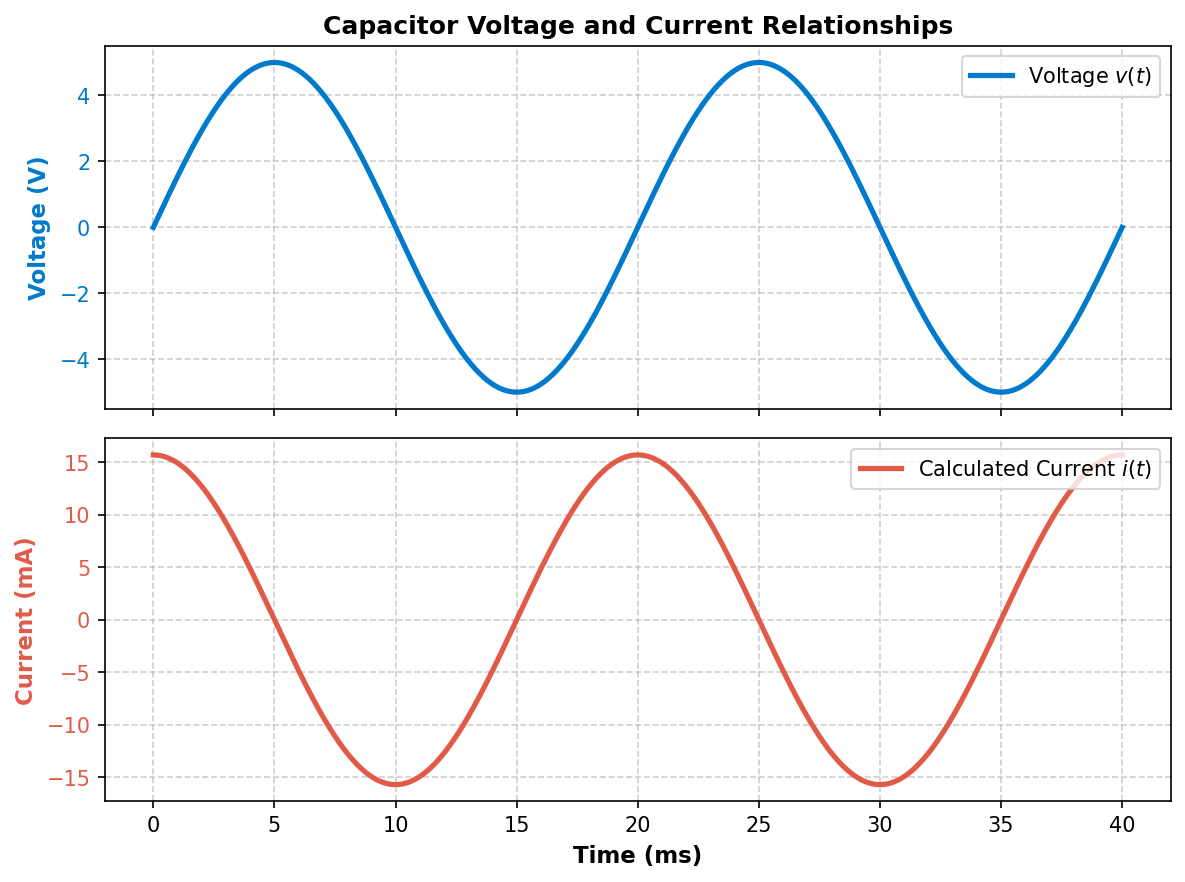
\includegraphics[height=0.58\textheight]{../images/chapter13/capacitor_ac_voltage_current.png}
    \end{center}

    \vspace{1mm}
    {\scriptsize Steepest voltage climb $\to$ peak current. Voltage at
    its flat peak $\to$ current drops to zero.}
\end{frame}

\begin{frame}[fragile]{EE Focus: Checking the Bench Recording}
    \leavevmode
    \small
    The bench recording's \texttt{current\_mA} column was measured
    \emph{independently}. Differentiate the voltage and compare:

\begin{lstlisting}
C = 100e-6
t = np.arange(0, 2.001, 0.02)
v = 12.0 * np.exp(-t / 0.47)
i_measured = (v / 4700.0) * 1000

i_from_slope = -C * np.gradient(v, t) * 1000
\end{lstlisting}

    \begin{alertblock}{Result}
        \texttt{i\_measured[0] = 2.5532 mA}, \texttt{i\_from\_slope[0]
        = 2.4996 mA} --- largest disagreement only $0.0536\,\text{mA}$.
    \end{alertblock}
\end{frame}

\begin{frame}{Why the Edges Disagree Most}
    \leavevmode
    \texttt{np.gradient()} estimates the slope at each interior point
    using samples on \alert{both} sides --- accurate. At the very first
    and last samples, there is no neighbour on one side, so it falls
    back to a one-sided difference --- less accurate.

    \vspace{3mm}
    \begin{block}{General lesson}
        Numerical derivatives are least trustworthy at the
        \alert{edges} of a recording.
    \end{block}

    \vspace{3mm}
    \begin{alertblock}{A final caution}
        Differentiation \alert{amplifies} noise --- a small wobble in
        $v$ becomes a large spike in $dv/dt$. This is why data-quality
        work (Chapter~11) comes \emph{before} this chapter.
    \end{alertblock}
\end{frame}

\begin{frame}{Integration: Building Up a Total}
    \leavevmode
    \small
    \texttt{np.trapz(y, x)} applies the trapezoidal rule to an entire
    array at once. \texttt{np.cumsum()} builds a \alert{running total}
    step by step:

    \vspace{2mm}
    \begin{center}
    \texttt{[1, 2, 3]} $\xrightarrow{\texttt{np.cumsum()}}$ \texttt{[1,
    3, 6]}
    \end{center}

    \vspace{3mm}
    Multiplying that running total by the time step $dt$ turns it into
    a running approximation of the integral at \alert{every instant},
    not just the final total.
\end{frame}

\begin{frame}[fragile]{Application: Capacitor Charge from a Current Signal}
    \leavevmode
    \[
    v(t) = \frac{1}{C}\int i(t)\,dt
    \]
    A steady $2\,\text{mA}$ DC current into a $10\,\mu\text{F}$
    capacitor for $50\,\text{ms}$:

\begin{lstlisting}
C = 10e-6
t = np.linspace(0, 0.05, 1000)
dt = t[1] - t[0]
i = np.ones_like(t) * 0.002

accumulated_current = np.cumsum(i) * dt
v = (1 / C) * accumulated_current
\end{lstlisting}
\end{frame}

\begin{frame}{Charging a Capacitor: Constant Current, Linear Ramp}
    \leavevmode
    \begin{center}
    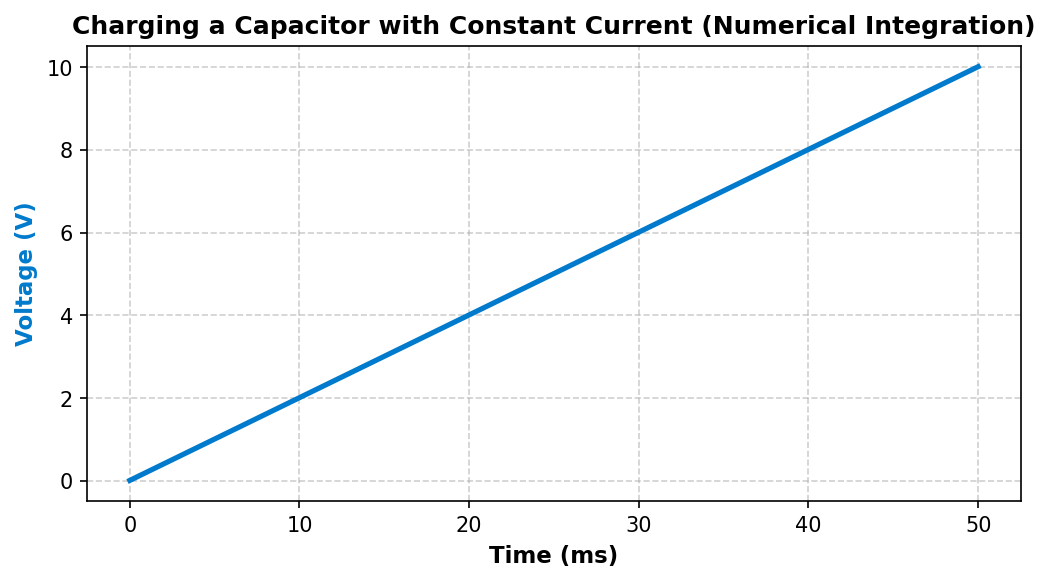
\includegraphics[height=0.58\textheight]{../images/chapter13/capacitor_charging_cumsum.png}
    \end{center}

    \vspace{1mm}
    {\scriptsize Because the current is constant, the charge
    accumulates at a perfectly steady rate --- the voltage climbs as a
    straight, linear ramp.}
\end{frame}

\begin{frame}[fragile]{Verifying \texttt{np.trapz()} Against an Exact Integral}
    \leavevmode
    $y = x^2$ over $[0, 10]$, whose exact integral you already know:

\begin{lstlisting}
x = np.linspace(0, 10, 1000)
y = x**2
area = np.trapz(y, x)
print("Approximate area:", area)
# Approximate area: 333.333500333834
\end{lstlisting}

    \vspace{2mm}
    \[
    \int_0^{10} x^2\,dx = \left.\frac{x^3}{3}\right|_0^{10} = 333.33
    \]

    \begin{block}{Agreement}
        $333.3335$ (numerical) vs.\ $333.33$ (exact) --- confirms the
        trapezoidal rule's accuracy for fine sampling.
    \end{block}
\end{frame}

\begin{frame}[fragile]{Bridge: Slopes and Sums, Before Calculus Has a Name}
    \leavevmode
    \small
    Subtraction for a rate, addition for a total --- a battery charging
    with a tapering current:

\begin{lstlisting}
t = np.array([0, 1, 2, 3, 4, 5])
I = np.array([2.0, 2.0, 1.6, 1.2, 0.8, 0.4])

Q = np.cumsum(I)       # ADDITION -> accumulates charge
dq = np.diff(Q)        # SUBTRACTION -> recovers the rate
\end{lstlisting}

    \begin{alertblock}{Not a coincidence}
        \textbf{Addition} turned a rate into a total --- exactly what
        an \alert{integral} does. \textbf{Subtraction} turned the total
        back into a rate --- exactly what a \alert{derivative} does.
    \end{alertblock}
\end{frame}

\begin{frame}{Predict Before You Run}
    \leavevmode
    In the AC capacitor example, the supply frequency is
    $50\,\text{Hz}$.

    \vspace{3mm}
    \begin{block}{Before changing any code}
        Predict what happens to the \alert{peak capacitor current} if
        the frequency is doubled to $100\,\text{Hz}$, using
        $i(t)=C\,dv/dt$ with $v(t)=5\sin(2\pi f t)$.
    \end{block}

    \vspace{3mm}
    Then change \texttt{f} in the code and check whether the peak
    current matched your prediction.
\end{frame}

%===============================================================================
\section{From Signals to System Models}
%===============================================================================

\begin{frame}{Why Polynomials, Here?}
    \leavevmode
    The first half of this chapter used derivatives and integrals to
    describe how a \alert{measured signal} changes and accumulates over
    time.

    \vspace{3mm}
    \begin{alertblock}{The shift}
        Engineers usually do not work with a raw signal forever ---
        they want a compact \alert{model} of the system that produced
        it. Many circuit and mechanical systems are described by a
        polynomial equation relating input to output.
    \end{alertblock}

    \vspace{3mm}
    Differentiating or integrating that polynomial tells you how the
    system responds to change, and its \alert{roots} reveal whether the
    system is stable.

    \vspace{2mm}
    {\small The rest of this chapter builds the polynomial tools for
    exactly that: representing, evaluating, and using them to check a
    system's frequency response and stability.}
\end{frame}

\begin{frame}{What Is a Polynomial?}
    \leavevmode
    \[
    a_N x^N + a_{N-1} x^{N-1} + \cdots + a_2 x^2 + a_1 x^1 + a_0 x^0
    \]
    $N+1$ terms; the variable's power increases from $0$ (right) to $N$
    (left). The values $a_N, \ldots, a_0$ are the \alert{coefficients}.

    \vspace{3mm}
    \begin{block}{Common applications in electrical engineering}
        \small
        \begin{itemize}
            \item System representation (Laplace-domain transfer
                  functions, $s$ as the variable)
            \item System stability evaluation
            \item Modelling acquired data
            \item Calibration
        \end{itemize}
    \end{block}
\end{frame}

\begin{frame}{Representing a Polynomial as a Vector}
    \leavevmode
    \small
    Coefficients, stored in order of \alert{decreasing powers}:

    \vspace{2mm}
    \begin{center}
    \begin{tabular}{@{}clc@{}}
        \toprule
        \textbf{No} & \textbf{Polynomial} & \textbf{Vector} \\
        \midrule
        1 & $3x^4 + x^3 - 2x^2 + 0.5x + 1$ & $[3,\ 1,\ -2,\ 0.5,\ 1]$ \\
        2 & $x - 1$ & $[1,\ -1]$ \\
        4 & $8$ & $[8]$ \\
        6 & $1 - 2x - 3x^2$ & $[-3,\ -2,\ 1]$ \\
        \bottomrule
    \end{tabular}
    \end{center}

    \vspace{2mm}
    {\scriptsize Missing terms get a coefficient of 0 --- the vector
    always has $N+1$ entries for a degree-$N$ polynomial.}
\end{frame}

\begin{frame}{Five Key NumPy Polynomial Functions}
    \leavevmode
    \begin{center}
    \begin{tabular}{@{}ll@{}}
        \toprule
        \textbf{Function} & \textbf{Description} \\
        \midrule
        \texttt{numpy.polymul()} & Polynomial multiplication \\
        \texttt{numpy.polydiv()} & Polynomial division \\
        \texttt{numpy.polyval()} & Polynomial evaluation \\
        \texttt{numpy.roots()}   & Polynomial roots \\
        \texttt{numpy.polyfit()} & Polynomial curve fitting \\
        \bottomrule
    \end{tabular}
    \end{center}
\end{frame}

\begin{frame}[fragile]{Multiplying and Dividing Polynomials}
    \leavevmode
    $p_1(x) = 2x^2 + 3x + 4$, \quad $p_2(x) = x + 2$:

\begin{lstlisting}
p1 = [2, 3, 4]
p2 = [1, 2]

result = np.polymul(p1, p2)
# [ 2  7 10  8]

quotient, remainder = np.polydiv(p1, p2)
# Quotient: [ 2. -1.]   Remainder: [6.]
\end{lstlisting}
\end{frame}

\begin{frame}{System Representation: The Laplace ``Recipe''}
    \leavevmode
    \small
    A \alert{transfer function} $Q(s) = Q_n/Q_d$ is a ``system
    recipe'': two polynomials whose coefficients summarize how a
    circuit, amplifier, or filter responds.

    \vspace{2mm}
    \begin{block}{What Python already gives you}
        \begin{itemize}
            \item Coefficients of $Q_n$, $Q_d$ are just list elements
            \item \texttt{np.roots(Q\_d)} checks \alert{stability}
            \item \texttt{np.polyval()} evaluated across a frequency
                  range produces a \alert{Bode-style} frequency
                  response
        \end{itemize}
    \end{block}

    \vspace{2mm}
    {\scriptsize You do not need to derive $s$ or solve a differential
    equation to use this.}
\end{frame}

\begin{frame}[fragile]{Worked Example: PID Motor Control}
    \leavevmode
    \small
    Motor $H(s) = \dfrac{1}{s-2}$, PID gains $P=4$, $D=2$, $I=1$:

\begin{lstlisting}
P, D, I = 4, 2, 1
H_n = [1]
H_d = [1, -2]
G_n = [D, P, I]
G_d = [1, 0]

Q_n = np.polymul(G_n, H_n)   # [2 4 1]
Q_d = np.polymul(G_d, H_d)   # [ 1 -2  0]
\end{lstlisting}
\end{frame}

\begin{frame}[fragile]{Polynomial Evaluation}
    \leavevmode
    Find $f(x) = 2x^2 + 4x + 1$ for $x = 3$:

\begin{lstlisting}
coefficients = [2, 4, 1]
result = np.polyval(coefficients, 3)
print("P(3) =", result)  # P(3) = 31
\end{lstlisting}

    \vspace{3mm}
    \begin{block}{Why this matters}
        Evaluating a polynomial over a whole \alert{range} of values
        --- not just one --- is exactly how a frequency response or a
        trajectory plot is produced.
    \end{block}
\end{frame}

%===============================================================================
\section{Frequency Response and Roots}
%===============================================================================

\begin{frame}[fragile]{Producing a Frequency Response}
    \leavevmode
    \small
    $s = j2\pi F$; evaluate $Q(s) = Q_n(s)/Q_d(s)$ over a range of $F$:

\begin{lstlisting}
Q_n = [2, 4, 1]
Q_d = [1, -2, 0]

frequencies = np.logspace(-3, 4, 1000)
omega = 2 * np.pi * frequencies
s = 1j * omega

Q_s = np.polyval(Q_n, s) / np.polyval(Q_d, s)
\end{lstlisting}
\end{frame}

\begin{frame}{The Frequency Response Plot}
    \leavevmode
    \begin{center}
    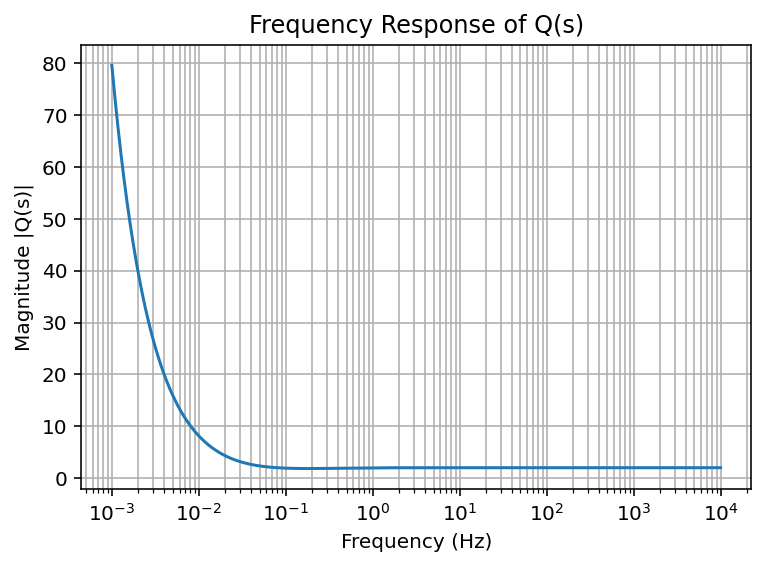
\includegraphics[height=0.62\textheight]{../images/chapter13/frequency_response.png}
    \end{center}

    \vspace{1mm}
    {\scriptsize This is the same technique behind a \alert{Bode plot}
    --- how electrical engineers visualize an amplifier, filter, or
    controller's response across frequency.}
\end{frame}

\begin{frame}[fragile]{Polynomial Roots}
    \leavevmode
    The roots of $P(x)$ are every $x$ where $P(x) = 0$. A degree-$N$
    polynomial has $N$ roots.

\begin{lstlisting}
coefficients = [1, 1, -4, -4]   # x^3 + x^2 - 4x - 4
roots = np.roots(coefficients)
print("Roots:", roots)
# Roots: [ 2. -2. -1.]
\end{lstlisting}
\end{frame}

\begin{frame}[fragile]{Worked Example: Vertical Displacement}
    \leavevmode
    \small
    $d = vt + \frac{g}{2}t^2$, $v = 30\,\text{m/s}$, $g =
    -9.8\,\text{m/s}^2$ --- when does the object hit the ground?

\begin{lstlisting}
v, g = 30, -9.8
p = [g/2, v, 0]

r = np.roots(p)
tground = r[r != 0][0]   # the non-zero root
\end{lstlisting}

    \vspace{2mm}
    \texttt{np.roots} finds \alert{when}; \texttt{np.polyval} computes
    the displacement at \alert{every other instant} so the trajectory
    can be plotted.
\end{frame}

\begin{frame}{The Trajectory}
    \leavevmode
    \begin{center}
    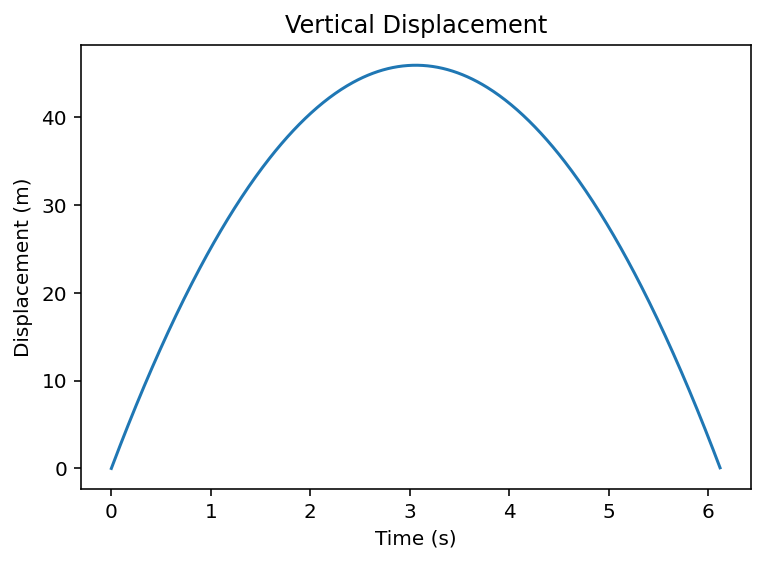
\includegraphics[height=0.6\textheight]{../images/chapter13/vertical_displacement.png}
    \end{center}
\end{frame}

\begin{frame}{System Stability: The Rule}
    \leavevmode
    A system represented by $Q(s) = Q_n/Q_d$ is \alert{stable} exactly
    when every root of the denominator $Q_d$ has a \alert{negative real
    part}.

    \vspace{3mm}
    \begin{columns}[t]
        \begin{column}{.48\textwidth}
            \begin{block}{Stable}
                \small All real parts of the roots are negative.
            \end{block}
        \end{column}
        \begin{column}{.48\textwidth}
            \begin{alertblock}{Not stable}
                \small Any root has a real part that is zero or
                positive.
            \end{alertblock}
        \end{column}
    \end{columns}

    \vspace{3mm}
    {\small A root with a positive real part means the response grows
    without bound after a disturbance.}
\end{frame}

\begin{frame}[fragile]{Worked Example: Checking Stability}
    \leavevmode
    \scriptsize
\begin{lstlisting}
def check_stability(C, Pn, Pd):
    Gn = [C[2], C[0], C[1]]
    Gd = [1, 0]
    Hn = np.polymul(Gn, Pn)
    Hd = np.polymul(Gd, Pd)
    Hd = np.polynomial.polynomial.polyadd(Hd, Hn)
    roots = np.roots(Hd)
    stable_roots = roots[roots.real >= 0]
    print("Stable" if len(stable_roots) == 0 else "Not stable")
\end{lstlisting}

    \vspace{1mm}
    \begin{center}
    \begin{tabular}{@{}lll@{}}
        \toprule
        \textbf{Call} & \textbf{Roots} & \textbf{Result} \\
        \midrule
        \texttt{check\_stability([4,1,0],[1],[1,-2])} & $0.17\pm0.55j$ & Not stable \\
        \texttt{check\_stability([3,3,3],[1,0],[1,1])} & $-0.50\pm0.71j$ & Stable \\
        \bottomrule
    \end{tabular}
    \end{center}
\end{frame}

\begin{frame}{Where This Chapter Leaves You}
    \leavevmode
    \small
    \begin{itemize}
        \item Rates and totals from \alert{measured data}: \texttt{np.diff()},
              \texttt{np.gradient()}, \texttt{np.trapz()},
              \texttt{np.cumsum()}.
        \item Polynomials as \alert{coefficient vectors}: multiply,
              divide, evaluate, find roots.
        \item A Laplace-domain transfer function is just \alert{two
              coefficient vectors} --- \texttt{np.roots()} on the
              denominator tells you if the system is stable;
              \texttt{np.polyval()} across a frequency range gives you
              a Bode-style response.
    \end{itemize}

    \vspace{4mm}
    \begin{center}
        \large\color{primary}\textbf{Next: Data Analytics and a First
        Look at Machine Learning}
    \end{center}
\end{frame}

\end{document}
